% Practice Test 15 — Texas Edition
% Questions: 30 (20 MC + 10 SA)
% Generated by scripts/generate_practice_tests.py

\begin{practiceQuestion}{1-3-q07}{mc}
\begin{questionText}
The table shows hours worked and money earned. What is $k$ and what does it mean?

\begin{center}
\begin{tabular}{|c|c|}
\hline \textbf{Hours} & \textbf{Earnings (\$)} \\ \hline $\frac{1}{2}$ & $\$6$ \\ $1$ & $\$12$ \\ $3$ & $\$36$ \\ \hline
\end{tabular}
\end{center}
\end{questionText}
\choiceA{$k = 6$; earns $\$6$ per half hour}
\choiceB{$k = 12$; earns $\$12$ per hour}
\choiceC{$k = 36$; earns $\$36$ per $3$ hours}
\choiceD{$k = 3$; works $3$ hours per $\$36$}
\correctAnswer{B}
\explanation{$k = \frac{6}{0.5} = 12$ or $\frac{12}{1} = 12$ or $\frac{36}{3} = 12$. The unit rate is $\$12$ per hour.}
\end{practiceQuestion}

\begin{practiceQuestion}{1-6-q03}{mc}
\begin{questionText}
A car travels $210$ miles on $6$ gallons of gas. How far can it go on $10$ gallons?
\end{questionText}
\choiceA{$300$ miles}
\choiceB{$330$ miles}
\choiceC{$350$ miles}
\choiceD{$360$ miles}
\correctAnswer{C}
\explanation{Unit rate: $210 \div 6 = 35$ mpg. On $10$ gallons: $35 \times 10 = 350$ miles.}
\end{practiceQuestion}

\begin{practiceQuestion}{2-1-q18}{mc}
\begin{questionText}
Mia scored $85\%$ on a test with $60$ questions. How many questions did she answer correctly?
\end{questionText}
\choiceA{$48$}
\choiceB{$50$}
\choiceC{$51$}
\choiceD{$54$}
\correctAnswer{C}
\explanation{$85\% = 0.85$. Multiply: $0.85 \times 60 = 51$ questions correct.}
\end{practiceQuestion}

\begin{practiceQuestion}{2-3-q18}{mc}
\begin{questionText}
A bakery sold $160$ cupcakes on Monday and $200$ cupcakes on Tuesday. What is the percent increase from Monday to Tuesday?


\numberLine[5]{160}{205}
\end{questionText}
\choiceA{$20\%$}
\choiceB{$25\%$}
\choiceC{$30\%$}
\choiceD{$40\%$}
\correctAnswer{B}
\explanation{Change: $200 - 160 = 40$. Percent increase: $40 \div 160 = 0.25 = 25\%$.}
\end{practiceQuestion}

\begin{practiceQuestion}{2-6-q24}{sa}
\begin{questionText}
What principal do you need to deposit at $4\%$ simple interest to earn $\$360$ in $3$ years?
\end{questionText}
\correctAnswer{$\$3{,}000$}
\explanation{$360 = P \times 0.04 \times 3$ → $360 = 0.12P$ → $P = \$3{,}000$.}
\end{practiceQuestion}

\begin{practiceQuestion}{2-8-q15}{mc}
\begin{questionText}
You charge $\$400$ on a credit card at $10\%$ annual interest. You pay $\$200$ right away and owe $\$200$ for $1$ year. How much total interest do you pay?
\end{questionText}
\choiceA{$\$40$}
\choiceB{$\$20$}
\choiceC{$\$10$}
\choiceD{$\$60$}
\correctAnswer{B}
\explanation{You owe $\$200$ for $1$ year. Interest $= 200 \times 0.10 = \$20$.}
\end{practiceQuestion}

\begin{practiceQuestion}{2-9-q24}{sa}
\begin{questionText}
Name one advantage of investing and one advantage of a savings account.
\end{questionText}
\correctAnswer{Investing: higher potential growth; Savings: low risk}
\explanation{Investments can grow faster but carry risk. Savings accounts are safe but earn less.}
\end{practiceQuestion}

\begin{practiceQuestion}{2-10-q20}{sa}
\begin{questionText}
$\$900$ at $10\%$ simple interest for $3$ years. What is the total interest earned?
\end{questionText}
\correctAnswer{$\$270$}
\explanation{$I = 900 \times 0.10 \times 3 = \$270$.}
\end{practiceQuestion}

\begin{practiceQuestion}{4-1-q28}{gmc}
\begin{questionText}
Look at the input-output table below.

\begin{center}
\begin{tikzpicture}[scale=0.8]
  \node[draw, rounded corners, fill=funOrange!20, minimum width=2.5cm, minimum height=1cm] at (3,0) {\textbf{Rule: ?}};
  \draw[->, thick] (0,0) -- (1.5,0);
  \draw[->, thick] (4.5,0) -- (6,0);
  \node[left] at (0,0) {\textbf{Input}};
  \node[right] at (6,0) {\textbf{Output}};
  % Table
  \node at (0,-1.5) {$1$}; \node at (6,-1.5) {$5$};
  \node at (0,-2.2) {$2$}; \node at (6,-2.2) {$9$};
  \node at (0,-2.9) {$3$}; \node at (6,-2.9) {$13$};
  \node at (0,-3.6) {$4$}; \node at (6,-3.6) {$17$};
\end{tikzpicture}
\end{center}

Which expression represents the rule?
\end{questionText}
\choiceA{$x + 4$}
\choiceB{$5x$}
\choiceC{$4x + 1$}
\choiceD{$3x + 2$}
\correctAnswer{C}
\explanation{Test $x = 1$: $4(1) + 1 = 5$ \checkmark. Test $x = 2$: $4(2) + 1 = 9$ \checkmark. The rule is $4x + 1$.}
\end{practiceQuestion}

\begin{practiceQuestion}{4-2-q24}{sa}
\begin{questionText}
Simplify $-3.5y + 2.1 + 1.5y - 0.6$.
\end{questionText}
\correctAnswer{$-2y + 1.5$}
\explanation{Combine variable terms: $-3.5y + 1.5y = -2y$. Combine constants: $2.1 - 0.6 = 1.5$. Result: $-2y + 1.5$.}
\end{practiceQuestion}

\begin{practiceQuestion}{5-3-q17}{mc}
\begin{questionText}
Solve $-3(2n + 4) = -24$.
\end{questionText}
\choiceA{$n = 6$}
\choiceB{$n = -2$}
\choiceC{$n = 2$}
\choiceD{$n = 4$}
\correctAnswer{C}
\explanation{Divide by $-3$: $2n + 4 = 8$. Subtract $4$: $2n = 4$. Divide by $2$: $n = 2$. Check: $-3(2(2)+4) = -3(8) = -24$ \checkmark.}
\end{practiceQuestion}

\begin{practiceQuestion}{5-4-q09}{mc}
\begin{questionText}
Solve $1.2x + 0.8 = 4.4$.
\end{questionText}
\choiceA{$x = 3$}
\choiceB{$x = 4.33$}
\choiceC{$x = 3.6$}
\choiceD{$x = 2.5$}
\correctAnswer{A}
\explanation{Subtract $0.8$: $1.2x = 3.6$. Divide by $1.2$: $x = 3$. Check: $1.2(3) + 0.8 = 3.6 + 0.8 = 4.4$ \checkmark.}
\end{practiceQuestion}

\begin{practiceQuestion}{5-5-q15}{mc}
\begin{questionText}
A student needs at least $70$ points to pass a test. She earns $4$ points per question and has $10$ bonus points. Which inequality finds the minimum number of questions $q$ she must answer?
\end{questionText}
\choiceA{$4q + 10 > 70$}
\choiceB{$4q + 10 \geq 70$}
\choiceC{$4q - 10 \geq 70$}
\choiceD{$10q + 4 \geq 70$}
\correctAnswer{B}
\explanation{Score $= 4q + 10$, needs at least $70$: $4q + 10 \geq 70$.}
\end{practiceQuestion}

\begin{practiceQuestion}{5-6-q25}{sa}
\begin{questionText}
Solve $7x - 3 \geq 18$. Give the smallest integer that is a solution.
\end{questionText}
\correctAnswer{$x = 3$}
\explanation{Add $3$: $7x \geq 21$. Divide by $7$: $x \geq 3$. The smallest integer solution is $3$.}
\end{practiceQuestion}

\begin{practiceQuestion}{6-2-q26}{gmc}
\begin{questionText}
The original drawing below uses scale $1$ cm $= 10$ m. You are asked to redraw the rectangle at scale $1$ cm $= 5$ m. What will the new dimensions be?

\begin{center}
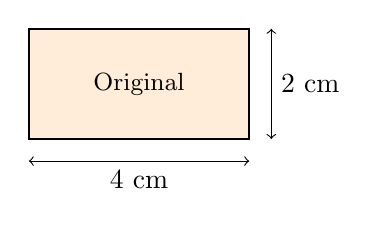
\begin{tikzpicture}[scale=0.7]
  \draw[thick,fill=orange!15] (0,0) rectangle (4,2);
  \draw[<->] (0,-0.4) -- (4,-0.4);
  \node[below] at (2,-0.4) {$4$ cm};
  \draw[<->] (4.4,0) -- (4.4,2);
  \node[right] at (4.4,1) {$2$ cm};
  \node at (2,1) {\small Original};
\end{tikzpicture}
\end{center}
\end{questionText}
\choiceA{$2$ cm by $1$ cm}
\choiceB{$4$ cm by $2$ cm}
\choiceC{$8$ cm by $4$ cm}
\choiceD{$20$ cm by $10$ cm}
\correctAnswer{C}
\explanation{Scale ratio: $\frac{10}{5} = 2$. New dimensions: $4 \times 2 = 8$ cm by $2 \times 2 = 4$ cm.}
\end{practiceQuestion}

\begin{practiceQuestion}{6-3-q22}{sa}
\begin{questionText}
Two sides of a triangle are $5$ cm and $5$ cm with an included angle of $60°$. What type of triangle is formed?
\end{questionText}
\correctAnswer{Equilateral triangle}
\explanation{Two equal sides with a $60°$ included angle gives a triangle where all angles are $60°$ (isosceles with $60°$ forces equilateral). All three sides are $5$ cm.}
\end{practiceQuestion}

\begin{practiceQuestion}{6-4-q03}{mc}
\begin{questionText}
Can a triangle have angles $50°$, $60°$, and $80°$?
\end{questionText}
\choiceA{Yes, because the angles are all positive}
\choiceB{Yes, because each angle is less than $180°$}
\choiceC{No, because $50 + 60 + 80 = 190 \neq 180$}
\choiceD{No, because the angles are not equal}
\correctAnswer{C}
\explanation{The three angles sum to $190°$, not $180°$. Triangle angles must always sum to exactly $180°$.}
\end{practiceQuestion}

\begin{practiceQuestion}{6-5-q06}{mc}
\begin{questionText}
You slice a cube with a vertical cut from one face to the opposite face, perpendicular to the base. What is the most likely cross-section shape?
\end{questionText}
\choiceA{Square or rectangle}
\choiceB{Circle}
\choiceC{Triangle}
\choiceD{Hexagon}
\correctAnswer{A}
\explanation{A vertical cut through a cube perpendicular to the base typically produces a rectangle. If the cut goes through the center parallel to a face, it can be a square.}
\end{practiceQuestion}

\begin{practiceQuestion}{6-8-q15}{mc}
\begin{questionText}
A model of a building uses scale $1:200$. The model is $0.3$ m tall. How tall is the real building?
\end{questionText}
\choiceA{$6$ m}
\choiceB{$30$ m}
\choiceC{$60$ m}
\choiceD{$600$ m}
\correctAnswer{C}
\explanation{$0.3 \times 200 = 60$ m.}
\end{practiceQuestion}

\begin{practiceQuestion}{7-4-q21}{sa}
\begin{questionText}
A figure is made of a semicircle with diameter $10$ cm and a rectangle $10$ cm by $6$ cm. What is the total area? Use $\pi \approx 3.14$.
\end{questionText}
\correctAnswer{$99.25$ cm$^2$}
\explanation{Rectangle: $10 \times 6 = 60$ cm$^2$. Semicircle: $\frac{1}{2} \times 3.14 \times 5^2 = \frac{1}{2} \times 78.5 = 39.25$ cm$^2$. Total: $60 + 39.25 = 99.25$ cm$^2$.}
\end{practiceQuestion}

\begin{practiceQuestion}{7-5-q24}{sa}
\begin{questionText}
A triangular prism has a right-triangle base with legs $3$ cm and $4$ cm. The prism is $12$ cm long. The hypotenuse of the triangle is $5$ cm. What is the total surface area?
\end{questionText}
\correctAnswer{$156$ cm$^2$}
\explanation{Two triangles: $2 \times \frac{1}{2} \times 3 \times 4 = 12$ cm$^2$. Three rectangles: $3 \times 12 + 4 \times 12 + 5 \times 12 = 36 + 48 + 60 = 144$ cm$^2$. Total: $12 + 144 = 156$ cm$^2$.}
\end{practiceQuestion}

\begin{practiceQuestion}{7-6-q13}{mc}
\begin{questionText}
If you triple the height of a rectangular prism while keeping the base the same, what happens to the volume?
\end{questionText}
\choiceA{It stays the same}
\choiceB{It doubles}
\choiceC{It triples}
\choiceD{It increases by a factor of $9$}
\correctAnswer{C}
\explanation{$V = Bh$. If $h$ becomes $3h$, then $V = B(3h) = 3Bh$. The volume triples.}
\end{practiceQuestion}

\begin{practiceQuestion}{8-1-q01}{mc}
\begin{questionText}
A school has $800$ students. The principal surveys $50$ students about their favorite subject. What is the population?
\end{questionText}
\choiceA{The $50$ surveyed students}
\choiceB{All $800$ students in the school}
\choiceC{The principal}
\choiceD{The students who like math}
\correctAnswer{B}
\explanation{The population is the entire group you want to study — all $800$ students.}
\end{practiceQuestion}

\begin{practiceQuestion}{8-2-q04}{mc}
\begin{questionText}
A random sample of $50$ customers at a store found that the average purchase was $\$32$. If the store has $1{,}200$ customers per day, predict the total daily sales.
\end{questionText}
\choiceA{$\$16{,}000$}
\choiceB{$\$32{,}000$}
\choiceC{$\$38{,}400$}
\choiceD{$\$60{,}000$}
\correctAnswer{C}
\explanation{$1{,}200 \times \$32 = \$38{,}400$.}
\end{practiceQuestion}

\begin{practiceQuestion}{8-4-q14}{mc}
\begin{questionText}
Data: $42, 45, 47, 50, 53, 55, 58$. Find $Q_1$ and $Q_3$.
\end{questionText}
\choiceA{$Q_1 = 45$, $Q_3 = 55$}
\choiceB{$Q_1 = 42$, $Q_3 = 58$}
\choiceC{$Q_1 = 47$, $Q_3 = 53$}
\choiceD{$Q_1 = 44$, $Q_3 = 56$}
\correctAnswer{A}
\explanation{Median $= 50$. Lower half: $42, 45, 47$, so $Q_1 = 45$. Upper half: $53, 55, 58$, so $Q_3 = 55$.}
\end{practiceQuestion}

\begin{practiceQuestion}{8-5-q10}{mc}
\begin{questionText}
In a stem-and-leaf plot, $8 \mid 0$ represents:
\end{questionText}
\choiceA{$8$}
\choiceB{$0.8$}
\choiceC{$80$}
\choiceD{$8.0$}
\correctAnswer{C}
\explanation{Stem $8$ with leaf $0$ means $80$.}
\end{practiceQuestion}

\begin{practiceQuestion}{8-6-q04}{mc}
\begin{questionText}
A circle graph shows that $40\%$ of $300$ students chose basketball as their favorite sport. How many students chose basketball?
\end{questionText}
\choiceA{$40$}
\choiceB{$100$}
\choiceC{$120$}
\choiceD{$160$}
\correctAnswer{C}
\explanation{$40\%$ of $300 = 0.40 \times 300 = 120$.}
\end{practiceQuestion}

\begin{practiceQuestion}{9-4-q29}{gsa}
\begin{questionText}
The bar graph shows the predicted number of times each color should appear if a spinner is spun $60$ times. Based on this model, what is the probability of landing on green? Write your answer as a fraction in simplest form.

\begin{center}
\begin{tikzpicture}[scale=0.55]
  \draw[thick,->] (0,0) -- (0,32) node[above,font=\small] {Predicted};
  \draw[thick,->] (0,0) -- (7,0);
  \foreach \y in {5,10,...,30} {
    \draw[gray!30] (0,\y) -- (6.5,\y);
    \node[left,font=\small] at (0,\y) {\y};
  }
  \fill[funRed!70] (0.5,0) rectangle (1.5,30);
  \fill[funBlue!70] (2.5,0) rectangle (3.5,18);
  \fill[funGreen!70] (4.5,0) rectangle (5.5,12);
  \node[below,font=\small] at (1,0) {Red};
  \node[below,font=\small] at (3,0) {Blue};
  \node[below,font=\small] at (5,0) {Green};
\end{tikzpicture}
\end{center}
\end{questionText}
\correctAnswer{$\frac{1}{5}$}
\explanation{Green is predicted to appear $12$ out of $60$ times. $P = \frac{12}{60} = \frac{1}{5}$.}
\end{practiceQuestion}

\begin{practiceQuestion}{9-6-q22}{sa}
\begin{questionText}
Two dice are rolled. What is the probability that the sum is exactly $6$? Write your answer as a fraction in simplest form.
\end{questionText}
\correctAnswer{$\frac{5}{36}$}
\explanation{Outcomes with sum $6$: $(1,5), (2,4), (3,3), (4,2), (5,1)$ — $5$ out of $36$. $P = \frac{5}{36}$.}
\end{practiceQuestion}

\begin{practiceQuestion}{9-7-q08}{mc}
\begin{questionText}
In a simulation, you roll a die $120$ times to model rolling a $5$. About how many times do you expect to roll a $5$?
\end{questionText}
\choiceA{$5$}
\choiceB{$12$}
\choiceC{$20$}
\choiceD{$60$}
\correctAnswer{C}
\explanation{$P(5) = \frac{1}{6}$. Expected: $120 \times \frac{1}{6} = 20$.}
\end{practiceQuestion}
